%'sine anatomia non sciemus' - Without anatomy there is no knowledge

%TODO
% Fix text
% add more information on fmri networks?
% talk more about evolution? [VINOD, MARS?]
\chapter{The Human Brain: An Introduction to Cytoarchitecture, Anatomy and Function}
\label{ch:intro_anato}

\section{Overview}
In this chapter we cover the basic aspects of cellular composition, morphology
and function of the human brain. We start with a brief introduction to the
human nervous system, in order to understand the biological context of the brain.
Then, we study the brain from both a microscopic and a macroscopic view. In the
microscopic view, we explain the cellular composition of the brain and how it’s
organized. In the macroscopic view, we zoom out and make a review of the most 
important divisions and anatomical landmarks of the brain. Finally, we describe
the functional role of some of these gross anatomical divisions. This chapter is
heavily based on the books: Neuroscience~\cite{Purves2004} ; Clinical
Neuroscience~\cite{Johns} and Atlas of Human Brain Connections~\cite{Catani2012}.
We encourage the reader to further deepen each subject using those books.

\section{The Human Nervous System}
Every organ in our body works as part of a larger system of organs interacting
towards a common goal. Our brain, the main actor of this thesis,
forms part of the nervous system, the system concerned with concious life.
The nervous system is the most complicated and highly organized of the various
systems which make up the human body\cite{Gray1918}. It is the mechanism
concerned with the analysis and integration of internal and external stimuli,
and with the reactions and adjustments of the organism in response to them. It
is anatomically divided into two parts, central and peripheral \ref{fig:cns_and_pns}.
The central nervous system (CNS) consist of the brain and the spinal cord. The
peripheral nervous system (PNS) consists of a series of nerves that link
receptors on the body with the central nervous system. These nerves are
associated with the functions of the special and general senses and with the
voluntary movements of the body. As a system, the PNS transmits stimuli from
the environment to circuits within the spinal cord and the brain, which are
integrated alongside internal stimuli in order to produce a response. This
response travels back trough the PNS and is translated into body movement or
the adjustment of internal organs (fig. \ref{fig:cns_and_pns}). 

\begin{figure}[h]
    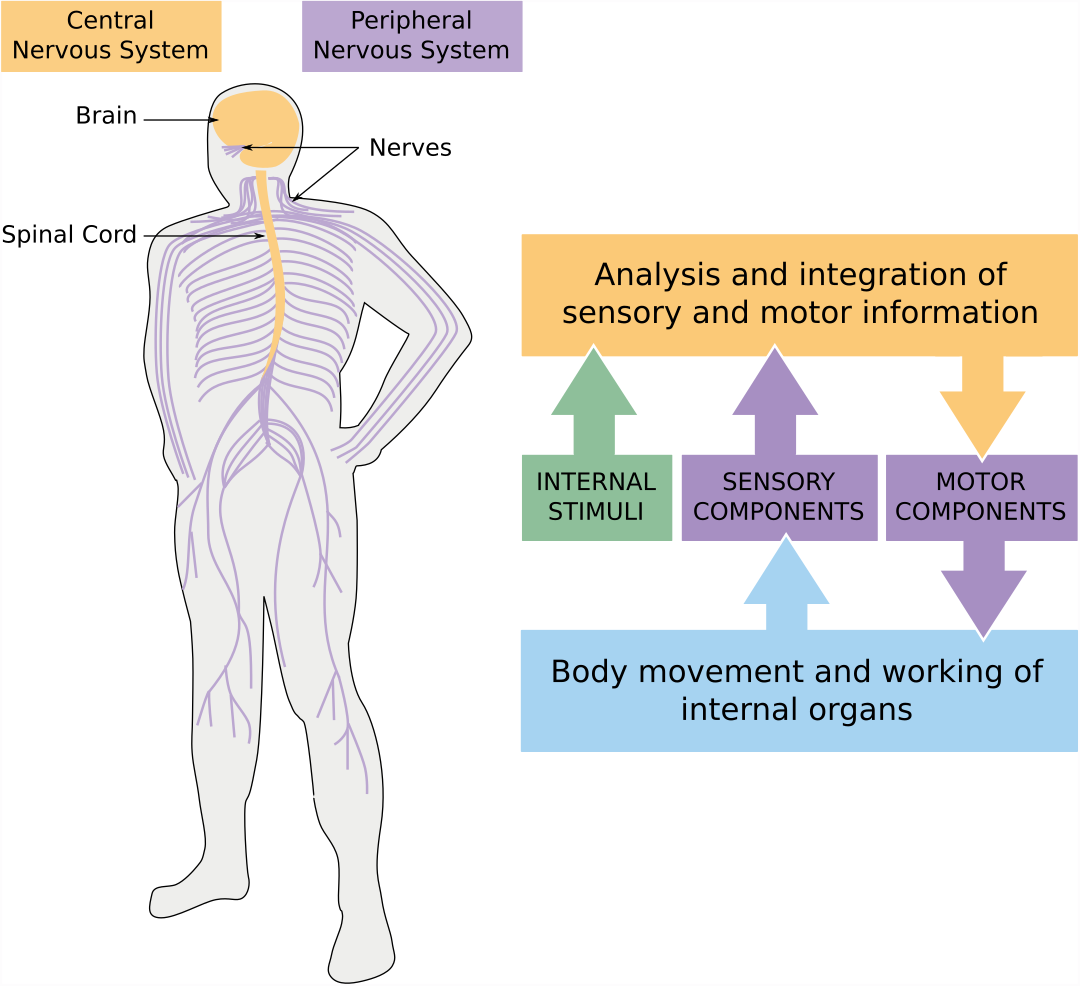
\includegraphics[width=0.49\textwidth]{2.neuroanatomy/img/pns_and_cns.png}
    \caption{The nervous system is anatomically divided in two: The central
             nervous system (CNS) and the peripheral nervous system (PNS).
             On the left we show a simplified representation of the CNS and
             PNS in the human body. On the right we schematize how these systems
             interact beween them: internal and external stimuli gathered by
             the PNS and sent to proccess to the CNS, which then decides how to
             respond. This image was adapted from the book Neuroscience~\cite{Johns}.}
    \label{fig:cns_and_pns}
\end{figure}  

In this thesis we will focus only on the brain. We start by talking about its
cellular composition and internal organization.

\section{A Microscopic View of the Human Brain}

\begin{figure*}[h!]
    \includegraphics[width=\textwidth, height=200px]{missing.png}
    \caption{Different types of neuronal and nonneuronal cells. (A) a pyramidal
             neuron, (B) granule neuron, (C) neuron with a highly complex
             arborization, (D) von Economo neuron. (E) Neuroglia, or supporting cell }
    \label{fig:neuron_types}
\end{figure*}

At a microscopical view, the human brain is composed by cells that can be
divided in two broad categories: nerve cells (or neurons), and supporting cells
called neuroglia (or simply glia). Nerve cells (Fig. \ref{fig:neuron_types} A)
are discrete entities that communicate with one another by means of specialized
contacts called “synapses”\cite{Purves2004}. Supporting cells (Fig. \ref{fig:neuron_types} E),
in contrast, are not capable of electrical signaling; nevertheless,
they have several essential functions in the developing and adult brain. The
human brain possess on average 86.06 +/- 8.12 billion neurons and
84.61 +/- 2.17 billion nonneuronal cells, making it a linearly scaled-up primate
brain in its cellular composition. In terms of distribution, 80\% of the neurons
are present in the cerebellum, and approximately all the rest are in the cortex.
Meanwhile 80\% of the nonneuronal cells are in the cortex, with almost all the
rest in the cerebellum.

% THIS NEED TO BE HERE TO MAINTAIN COHERENCE IN THE COMPILED PDF
% BUT IT'S ACTUALLY OF THE NEXT SECTION
\begin{figure*}[h!]
    \includegraphics[width=\textwidth, height=200px]{missing.png}
    \caption{Brain tissue can be divided into grey and white matter. (A) Grey matter
             is composed mainly of cell bodies. (B) White matter is made up mostly
             of packed axons.}
    \label{fig:white_grey_matter}
\end{figure*}
% 

\subsection{Neurons}

The basic cellular organization of neurons resembles that of other cells; however,
they are clearly distinguished by specialization for intercellular communication.
This attribute is apparent in their overall morphology, in the specific
organization of their membrane components for electrical signaling, and in the
structural intricacies of the contacts between neurons. The spectrum of neuronal
geometries ranges from a small minority of cells that lack dendrites altogether
to neurons with complex dendritic arborizations (i.e. Fig. \ref{fig:neuron_types} C).
The complexity of the dedritic arbor constrains the amount of neurons with who
a neuron can communicate, ranging from one or few, to a commensurately larger
number of other neurons.

From a functional point of view, we can distinguish two type of neurons:
excitatory and inhibitory. Excitatory neurons release the neurotransmitter
glutamate to send signals to other cells. Inhibitory neurons release
gamma-Aminobutryc acid, in order to reduce neuronal excitability throughout
the nervous system~\cite{Bekkers2011}.

From a morphologic point of view, neurons can be divided in two major types:
granule neurons and pyramidal neurons \cite{Purves2004}. Granule cells are 
star-shaped neurons with a typical diameter of less than 20$\mu$m. They are
multipolar neurons, this is, neurons that posses a single axon and many dendrites.
Granule cells are either excitatory or inhibitory, and mostly have purely
‘intrinsic’ axons, this is, they make only short-range, local connections~\cite{Purves2004}.
On the other hand, pyramidal neurons have large, pyramid-shape bodies that
range from 20-120$\mu$m. Pyramidal neurons are multipolar and excitatory neurons,
and they comprise about two-thirds of all neurons in the mammalian cerebral cortex.
On top of their numerical dominance, pyramidal neurons are also 'projection neurons',
meaning that they axons are often 'extrinsic', making long connections~\cite{Purves2004}.

Finally, neurons on a circuit can be classified based on their role in a 
neuronal circuit. Nerve cells that carry information toward the circuit are
called afferent neurons; nerve cells that carry information away from the 
circuit are called efferent neurons. Interneurons, or local circuit neurons,
only participate in the local aspects of a circuit.

%Another important type of neurons to this thesis are the spindle neurons \cite{Johns}.
%Spindle neurons, also called von Economo neurons (VENs), are a specific cfass of
%neurons that are characterized by a large spindle-shaped soma (or body),
%gradually tapering into a single apical axon in one direction, with only a
%single dendrite facing opposite. VENs emerged within the last decade as having
%a potentially major role in self-awareness and social cognition in humans \cite{Evrard2012}.

\begin{figure*}[h!]
    \includegraphics[width=\textwidth, height=200px]{missing.png}
    \caption{The cerebral cortex is characterize by its convoluted folds.
             Some landmarks are consistent across brains, as the central sulcus;
             lateral sulcus; parieto-occipital notch and pre-occipital notch.
             These landmarks help divide the hemispheres into lobes.}
    \label{fig:cortex_anatomy}
\end{figure*}

\subsection{Neuroglial}
Neuroglial cells are quite different from nerve cells. Glial cells do not
participate directly in synaptic interactions and electrical signaling, but
instead provide support to define synaptic contacts and maintain the signaling
abilities of neurons~\cite{Purves2004}. The term glia (from the Greek word
γλοιός meaning “glue”) reflects the nineteenth-century presumption that these
cells held the nervous system together in some way. The term has survived 
despite the lack of evidence that glia actually bind neurons together. Glial
roles that are well-established include maintaining the ionic milieu of nerve
cells, modulating the rate of nerve signal propagation, modulating synaptic
action by controlling the uptake of neurotransmitters at or near the synaptic
cleft, providing a scaffold for some aspects of neural development, and aiding
in the recovery from neural injury~\cite{Purves2004}.

\subsection{Neuronal Organization: Cortical Layers}

Brain cells are arranged in horizontal layers, or laminae~\cite{Waehnert2014}.
More than 90\% of the cerebral cortex has a characteristic six-layered composition\cite{RandS.SwensonM.D.2006}.
Layer I is the molecular
layer, which contains very few neurons; layer II the external granular layer;
layer III the external pyramidal layer; layer IV the internal granular layer;
layer V the internal pyramidal layer; and layer VI the multiform, or fusiform
layer. Each cortical layer contains different neuronal shapes, sizes and density
as well as different organizations of nerve fibers\cite{RandS.SwensonM.D.2006}.
The layer structure varies spatially in regard to cell organization (cytoarchitecture) and 
myelination (myeloarchitecture), defining distinct cortical areas which are
likely to perform different functions \cite{Waehnert2014, Bok1929}. 

Depending on the layers present, the cortex can be divided in agranular,
disgranular and granular regions\cite{Mesulam1982}. The agranular cortex is characterized by not
having a internal granule cell layer (layer IV). The granular cortex has two 
layers of granule cells, an external granular layer (II) and an internal granular
layer (IV). Dysgranular cortex has fewer granule cells, which are grouped in a
single layer or as distinct clusters.

The fine study of the cortical composition is called Cytoarchitectonics. We 
discuss the topic of parcelling the brain based on cytoarchitecture in chapter
4, now it's sufficient to say that the cerebral cortex is divided into more than
fifty regions based on its cellular composition under the microscope. The most
known and frequently cited cythoarchitectural organization is that of
Brodmann~\cite{Brodmann1909} (Fig. \ref{fig:brodmann_small}).

\begin{figure}[h]
    \includegraphics[width=0.49\textwidth, height=150px]{missing.png}
    \caption{The cerebral cortex is divided into more than 50 regions based on
             its cellular composition. Brodmann's\cite{Brodmann1909}
             parcellation is the most known and cited one.}
    \label{fig:brodmann_small}
\end{figure}

\section{A Macroscopic view of the Human Brain}
In the previous section, we talked about neurons and how they are specialized
to transmit information. Indeed, neurons never function in isolation; they are
organized into circuits or structures that process specific kinds of information.
The brain tissue comprises a diverse collection of these neural structures,
each with a distinctive shape and an intricate internal architecture.

Brain tissue can be divided into grey and white matter~\cite{Johns} (Fig. \ref{fig:white_grey_matter}).
Grey matter is composed mainly of neuronal cell bodies, dendrites and synapses.
It is sharply demarcated from the adjacent white matter, which is made up mostly
of axons travelling from grey matter to grey matter, or to other parts of the
nervous system. The pale colour of white matter is due to the lipid-rich myelin
sheath that surrounds axons and enhances their conduction velocity\cite{Johns}.

\begin{figure*}[h!]
    \includegraphics[width=\textwidth, height=200px]{missing.png}
    \caption{Major tracts in the white matter. Projection bundle: BLA. Other: BLA.
             OTHER: bla.}
    \label{fig:white_anatomy}
\end{figure*}

\subsection{Anatomy of the Grey Matter}

The grey matter is composed of: the cerebral cortex; the cerebellum; structures
within the white matter, called subcortical structures (i.e. thalamus; hypothalamus; etc),
and the grey column, which traverses the spinal cord. In this thesis we will
mainly focus on the cerebral cortex.

The cerebral cortex is the most important structure of the gray matter and
plays a major role in cognitive functions. It is a layered sheet of tissue,
2–3 millimetres thick, with highly convoluted folds. It's hypothesized that the
mechanical tension created by neuronal connections during development is a major
driving force of these folds~\cite{VanEssen1997}. An advantage of the folding
pattern, is that it allows to fit a large surface area within the available
cranial volume. In particular, the human cerebral cortex attains a surface area
of about 1600 $cm^2$, nearly three times what it would be in the absence of
convolutions~\cite{VanEssen1997}. The grooves and ridges created by this folding
process are called sulci and gyri respectively.

The cerebral cortex is divided in two hemispheres by a prominent central fissure.
The hemispheres are characterized by the gyri (singular, gyrus) or crests of
folded cortical tissue, and sulci (singular, sulcus) the grooves that divide
gyri from one another. Although gyral and sulcal patterns vary from individual
to individual, there are some fairly consistent landmarks, particularly the: 
central sulcus; lateral sulcus; parieto-occipital notch and pre-occipital notch.
These landmarks help divide the hemispheres into four lobes: occipital, 
temporal, parietal, and frontal. Hidden from surface view is the fifth lobe:
the insular lobe. Figure \ref{fig:cortex_anatomy} presents a illustration of this.

\subsection{Anatomy of the White Matter}
\begin{figure*}[h!]                                                                                                                    
    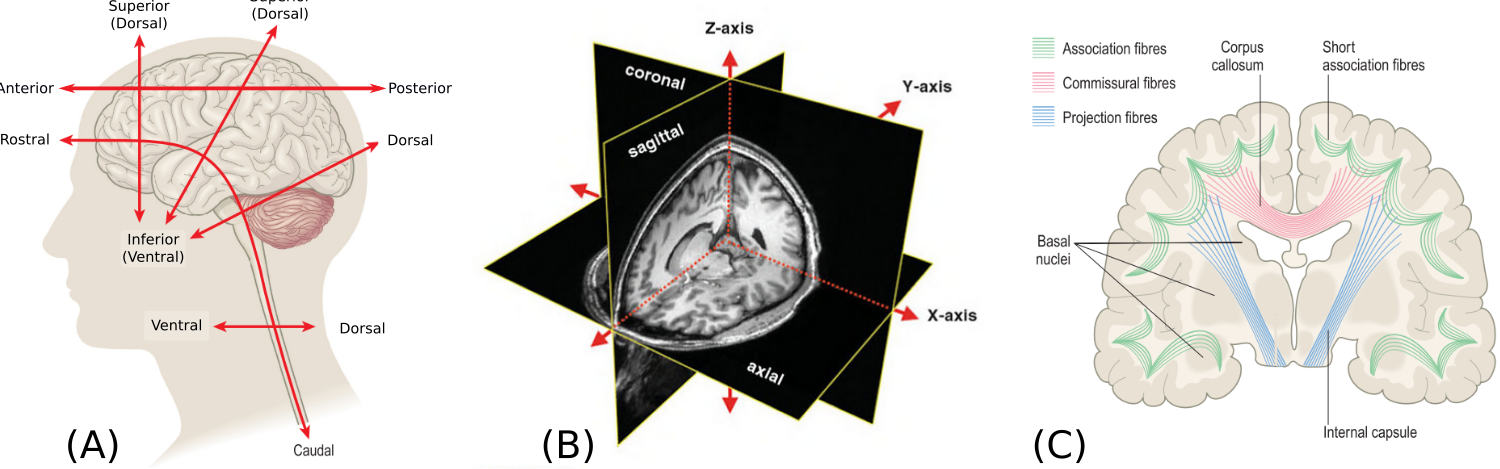
\includegraphics[width=\textwidth]{2.neuroanatomy/img/terminology.png}
    \caption{Terms commonly used to describe the orientation of the brain in surface (A), sectional (B) and connectional anatomy (C) representations.}
    \label{fig:anatomy_terminology}
\end{figure*}

Axons in the central nervous system are gathered into bundles of different
diameter, and several bundles form larger pathways called fasciculi, or tracts~\cite{Catani2012}.
Most of the cerebral fibers forming the white matter connect distant regions 
within the cortex. Others, connect cortical region with the peripherical nervous
system or subcortical structures. There are some fibers, the less, that connect
only subcortical structures.

Some of the major bundles running along the white matter are well defined in the
modern neuronanatomy. Examples of major bundles in the human brain are the
Corpus Callosum, the Internal Capusule and the Superior Longitudinal Fasciculus
(Fig. \ref{fig:white_anatomy}.)
The Corpus Callosum is the largest tract of the human brain, composed of some
200–300 million myelinated axons it connects both hemispheres, allowing to
transfer information from one to another~\cite{Catani2012}. The internal capsule
contain ascending fibres mainly from the thalamus to the cortex, and descending
fibres from the cortex to subcortical structures, and the spinal cord~\cite{Catani2012}.
This complex projection system conveys sensorial information to the cortex and 
controls movement. Our last example, the Inferior Longitudinal Fasciculus, is
a tract with long and short fibres connecting the occipital and temporal lobes~\cite{Catani2012}.
Its involved in visual and language functions.

\begin{figure*}[h!]                                                                                                                    
    \includegraphics[width=\textwidth,height=150px]{missing}
    \caption{(A) Different regions of the brain are specialized for different
             functions, most of them where mapped based on the postmortem 
             examination of brain lesions in subjects with functional
             deficiencies. (B) Closer look to the motor and sensory cortex.}
    \label{fig:brain_function}
\end{figure*}

\subsection{Neuroanatomical Naming Conventions}
In order to describe the location of structures on the brain, standardized
nomenclature is used. Brain's anatomy can be described from its surface,
from orthogonal sections that traverse the brain, or from its white matter~\cite{Catani2012}.

The surface of the brain can be viewed from the side (lateral view),
the middle (medial view), the front (anterior or frontal view), and the back
(posterior or occipital view)~\ref{fig:anatomy_terminology}. The same terminology
is used to indicate different regions of the brain surface (e.g. dorso-lateral prefrontral cortex).

Sectional neuroanatomy describes the relationship between cortical and
subcortical structures, most commonly visualized along orthogonal axial,
coronal, and sagital planes~\ref{fig:anatomy_terminology}. In radiological
convention, the axial slices are viewed from the feet towards the head.
The coronal planes are conventionally oriented with the left side of the brain
on the right side of the page (frontal view). Finally, the sagittal plane 
divides the brain into two hemispheres.

White-matter neuroanatomy delineates the origin, course, and termination of
connecting pathways~\ref{fig:anatomy_terminology}. The tracts are classified
according to their course and terminal projections. Commisural pathways run
along a horizontal axis and connect the two hemispheres. The majority of the
projection pathways have a perpendicular course along a dorso-ventral
(descending) or ventro-dorsal (ascending) axis and connect the cerebral
cortex to subcortical nuclei, cerebellum, and the spinal cord. The association
tracts run longitudinal along an antero-posterior axis and connect cortical 
areas within the same hemisphere.

These gross descriptions of some prominent anatomical landmarks provide a
framework for naming, locating and studying different brain structures. Being
able to locate brain regions in different subjects is a necessary first step
to study the basic of brain function.

\section{Brain Function}
While we know that concious emerges from the brain, we still have a long path
ahead to unravel how the brain works. So far, and thanks to the study of
brain lesions, many motor and cognitive functions have been mapped to coarse
brain regions (Fig. \ref{fig:brain_function}). In this section, we present an
overview of the general function attributed to each lobe, while introducing 
some of the functional subdivisions used later on this thesis.

\subsection{Frontal Lobe}
The frontal lobe is responsible for motor functions, speech production, 
planning, personality, insight and foresight.

One of its divisions, the precentral gyrus (Fig. \ref{fig:brain_function} A),
contains an inverted point-to-point map of the motor functions of the opposite
half of the body (Fig. \ref{fig:brain_function} B)~\cite{Johns, Purves2004,
Catani2012}. This area is called the primary motor cortex, and corresponds to
Brodmann's region 4. It was mapped by Penfield et al.~\cite{Penfield1954} trough
experimenting with electrical stimulation. A remarkable fact is that the area
allocated for each body part is proportional to the precision of movement
control~\cite{Johns}. In particular, the areas for the hands, face and tongue
are disproportionately large (Fig. \ref{fig:brain_function} B).

The region in front of the primary motor cortex is the lateral premotor area.
Defined as the Brodmann Area 6, it does not correspond to any particular gyral
or sulcal boundaries~\cite{Johns, Purves2004}. The premotor cortex also contains
an inverted body map and is concerned with preparation and execution of movement
sequences in response to external stimuli (as catching a ball, rather than throwing one)~\cite{Johns}.

The large portion of the frontal lobe anterior to the motor
and premotor areas is the prefrontal cortex and is involved in personality, 
behaviour, language and intellect~\cite{Johns}. Its mainly concerned with
organizing and planning behaviour in pursuit of short-, medium- and long-term goals.
It also has a cognitive inhibitory role, preventing inappropriate behaviour~\cite{Sigman2017}.

Finally, the opercular and triangular parts of the inferior frontal gyrus
(Brodmann Areas 44 and 45) correspond to Broca’s area. This area is involved in
the expressive aspects of spoken and written language (production of sentences
constrained by the rules of grammar and syntax)~\cite{Johns}. The area was named
after Pierre Paul Broca, who reported speach production impairments in two patients.
This area tends to be lateralized to the hemisphere in charge of the dominant
hand. 

\subsection{Parietal Lobe}
The parietal lobe is responsible for language comprehension, spatial orientation
and perception, and somatic senses, such as touch and temperature.

Located on the parietal lobe, immediately posterior to the centrar sulcus, and
parallel to the precentral gyrus, there is the postcentral gyrus. It corresponds 
to the primary somatosensory cortex (BA 3, 1 and 2). The sensory cortex contains
an inverted map of the opposite side of the body that mirrors that of the motor
cortex, but the relative proportions of the body parts reflect the degree of 
tactile sensitivity~\cite{Johns}.

\subsection{Occipital Lobe}
The occipital lobe is concerned entirely with visual processing and association.
It contains the Brodmann Area 17, which correspondes to the primary visual cortex.
The primary visual cortex is highly specialized for processing visual information, and
possess a point-to-point (retinotopic) representation of the visual field~\cite{Johns}.
The visual system continues in the visual association cortex (BA 18 and 19),
which helps in the detection of complex patterns and are believed to contribute
in detecting global motion~\cite{Johns, Purves2004}.

\subsection{Temporal Lobe}
The temporal lobe is involved in hearing, speech comprehension and visual recognition.

Contained by it is the auditory cortex (Fig. \ref{fig:cortex_anatomy}), which 
has a tonotopic map representing the audible frequency spectrum (low frequencies
laterally, high frequencies medially)~\cite{Johns}. More ventral is the fusiform
gyrus, which is involved in the recognition of complex visual patterns, as tools
or human faces~\cite{Saygin2011}. Another region, Wernicke’s area, corresponds to the 
posterior third of the superior temporal gyrus (Fig. \ref{fig:brain_function}) and
it's involved in language comprehension~\cite{Johns}. 

\subsection{Insula}
The insular cortex is hidden in the depths of the lateral sulcus (Fig.
\ref{fig:cortex_anatomy}). The insula is involved in attention, and in the
integration of sensory, affective, and cognitive cues~\cite{Bressler2010, Johns}.

\section{Brain Networks}

So far in this introduction to neuroanatomy, we have presented brain function
as studied by the modular paradigm.
In this paradigm, a discrete and continuous piece of cortical tissue is specialized
to serve one cognitive function or to represent one essential aspect of the
information processed by it~\cite{Fuster2000}. The interaction between many
of such modules would lead to complex cognitive function. However, accumulating
evidence shows that the paradigm has serious limitations. For example, lesions
in the brain almost never derive in the loss or degradation of only one cognitive
function~\cite{Fuster2000}. Furthermore, even the functions of primary sensory
areas, long standing thought as modular, appear to be part of a network that
integrates multisensory stimuli~\cite{Ghazanfar2006}.

A new paradigm is emerging in neuroscience, that moves beyond the simplistic
one to one mapping between cognitive functions and brain regions, and instead
maps cognitive functions to large-scale networks in the brain. So far, at least
8 major core functional networks have been defined\cite{Bressler2010}:
(i) a spatial attention network anchored in posterior parietal cortex and frontal eye fields;
(ii) a language network anchored in Wernicke’s and Broca’s areas;
(iii) an explicit memory network anchored in the hippocampal–entorhinal 
complex and inferior parietal cortex; (iv) a face-object recognition
network anchored in midtemporal and temporopolar cortices; (v) a
working memory-executive function network anchored in prefrontal and
inferior parietal cortices; (vi) central-executive network anchored in
dorsolateral prefrontal cortex and posterior parietal cortex; (vii) a salience
network anchored in anterior insula and anterior cingulate cortex; and (viii)
a default mode network, a set of functional networks that emerge while a person
is resting.

Thinking the brain as a set of interacting networks, instead of single anatomical
regions, creates a sound base to study cognition\cite{Bressler2010}. However,
if a single network can be said to support a specific cognitive function is 
still an open question in neuroscience. Answering it will depend on the 
developing of new techniques to study not only brain function, but also brain
connectivity.

\section{Conclusions}
This chapter introduced the basic knowledge in neuroanatomy necessary to
understand the rest of the thesis. Moreover, it explained how the interaction
between neurons by means of connectivity drives not only the brain morphology
but also its function. It also highlighted how neuroscience is moving from
viewing the brain as a mosaic of functionally specialized regions, to an
interactive network from which cognition arises. This view of the brain as 
a network is a key aspect that drives some of the contributions of this thesis.

Most of the knowledge content in this chapter comes from studies done on 
postmortem primate brains, or from results obtained with highly invasive
techniques. As with the modular paradigm, neuroscience is also moving forward
towards the use of non-invasive techniques. In the next chapter, we explain how 
advances in quantum physics helped to develop Magnetic Resonance Imaging (MRI),
which translated in a new era of non-invasive brain imaging.

\chapterbib
